\documentclass[a4paper,11pt]{article}
\usepackage[utf8]{inputenc}
\usepackage[french]{babel}
\usepackage{amsmath}
\usepackage[osf,sups]{Baskervaldx} % lining figures
\usepackage[bigdelims,cmintegrals,vvarbb,baskervaldx]{newtxmath} % math font
\usepackage{graphicx}
\usepackage{xcolor}
\usepackage{url,hyperref}

% margins
\setlength{\parindent}{0em}
\setlength{\parskip}{1em}
\addtolength{\hoffset}{-3.5em}
\addtolength{\textwidth}{7em}
\addtolength{\voffset}{-5em}
\addtolength{\textheight}{10em}


\begin{document}
\thispagestyle{empty}

{\bf
	Résolution de l'équation de Poisson par réseaux de neurones
}

{\bf Encadrants}:\\
Rafael Grompone von Gioi \verb+<rafael.grompone@ens-paris-saclay.fr>+\\
Enric Meinhardt-Llopis \verb+<enric.meinhardt@ens-paris-saclay.fr>+

{\bf Contexte}\\
Il y a trois techniques en calcul numérique qui sont bien différentes, mais qui
s'avèrent néanmoins formellement similaires.  D'abord, la {\bf factorisation}
d'une matrice pleine comme produit d'un nombre petit de matrices creuses.
C'est le cas par exemple de la Transformation de Fourier Rapide, où une matrice
pleine de taille~$2^N\times2^N$ s'écrit comme produit de~$N$ matrices creuses.
Seconde, les {\bf méthodes multigrid} pour la résolution d'une EDP, où la même
équation est résolue successivement à différents pas de
discrétisation---échelles---ce qui permet une convergence considérablement plus
rapide vers la solution globale.  Troisième, l'{\bf architecture U-Net} pour
les réseaux de neurones à convolution, où la pyramide multi-échelle d'une image
est analysée successivement par plusieurs couches convolutionnelles, puis les
résultats de chaque couche sont intégrés sur une image de sortie à la résolution
initiale.  Les réseaux de type U-Net sont une des briques de base du traitement
d'images moderne, et ils fournissent des résultats de l'état de l'art sur des
problèmes de classification, segmentation et debruitage d'images (REF: U-Net).

Si on vise à résoudre l'équation de Poisson~$\Delta u = f$ dans un domaine
rectangulaire, les deux premières techniques sont confondues, du au fait que la
transformée de Fourier discrète diagonalise l'opérateur Laplacien.
L'article (REF: article), paru récemment et devenu célèbre dans la communauté
de traiteurs de nuages de points, clôt le cercle et propose un réseau U-Net
pour résoudre l'équation de Poisson.

\begin{tabular}{ccc}
	\sf\color{blue} Multigrid PDE solvers&
	\sf\color{blue} Sparse matrix factorisation &
	\sf\color{blue} U-net ConvNets\\
	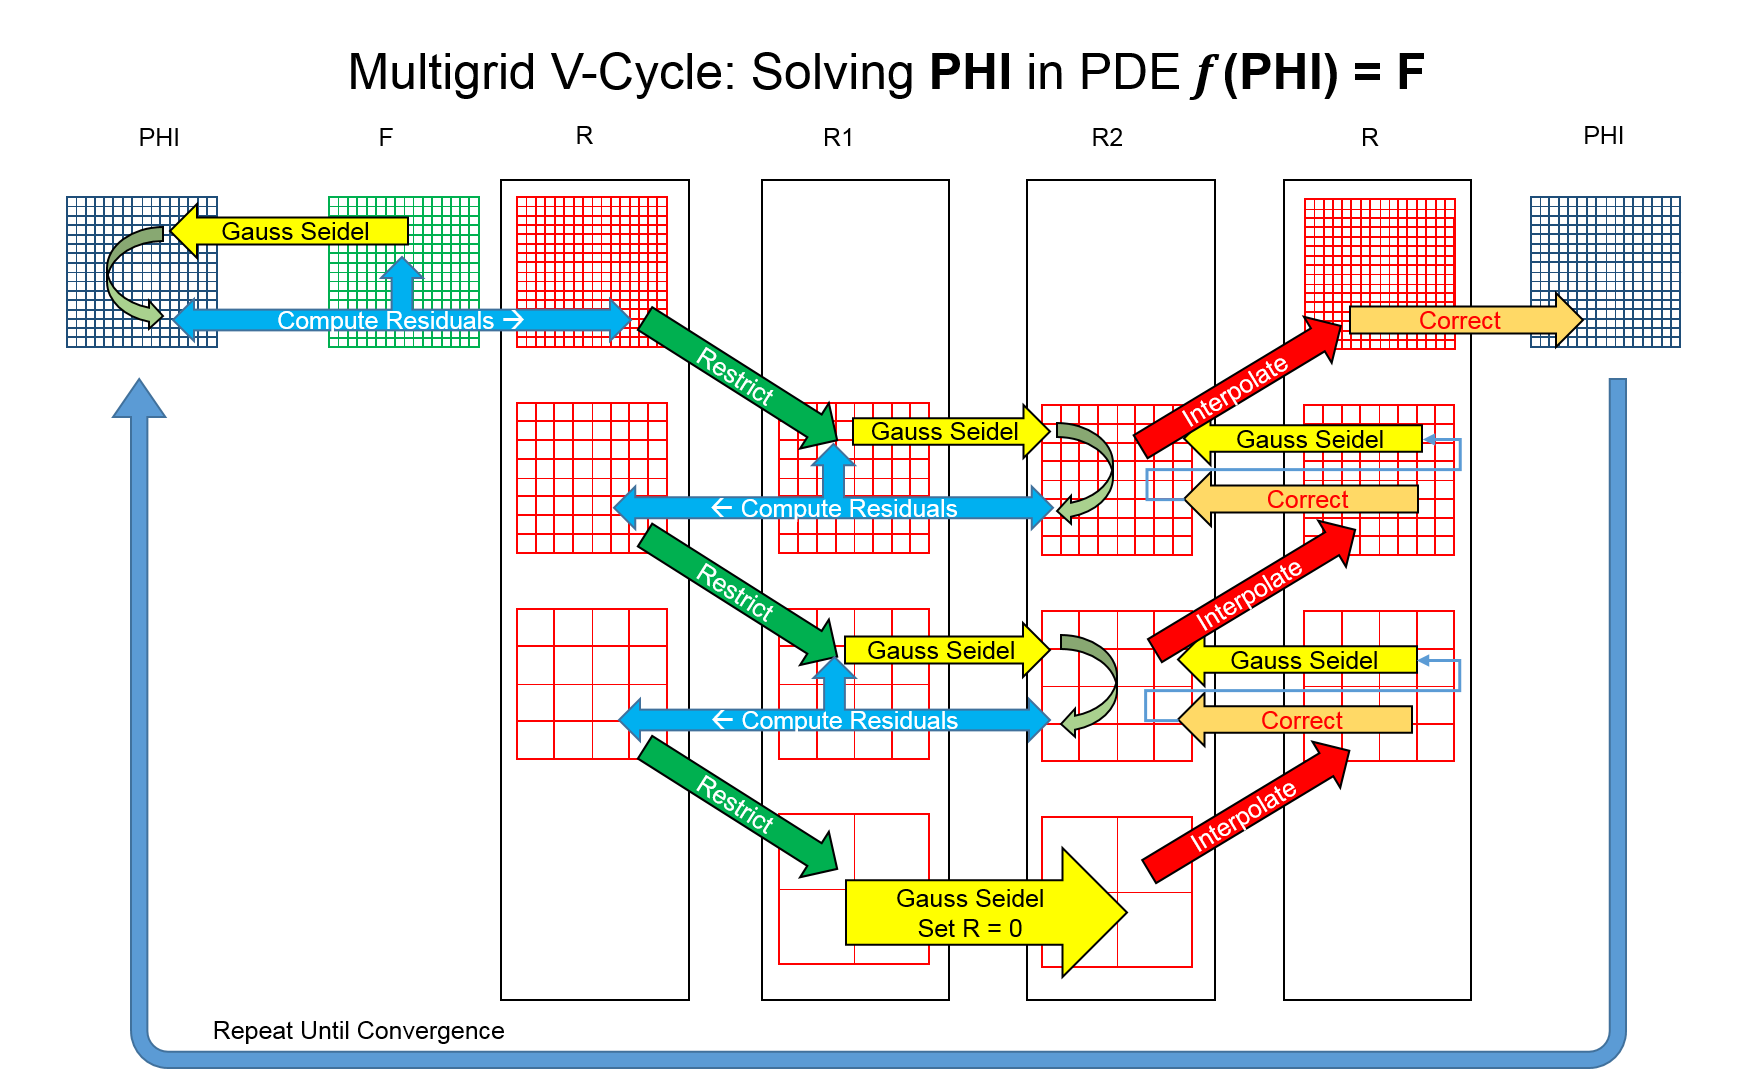
\includegraphics[width=0.3\linewidth]{f/multigrid.png} &
	%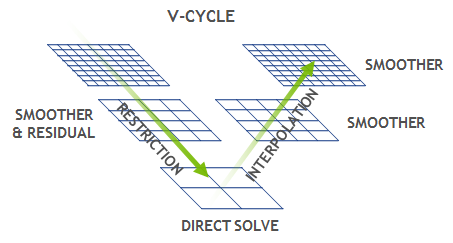
\includegraphics[width=0.32\linewidth]{f/vcycle.png} &
	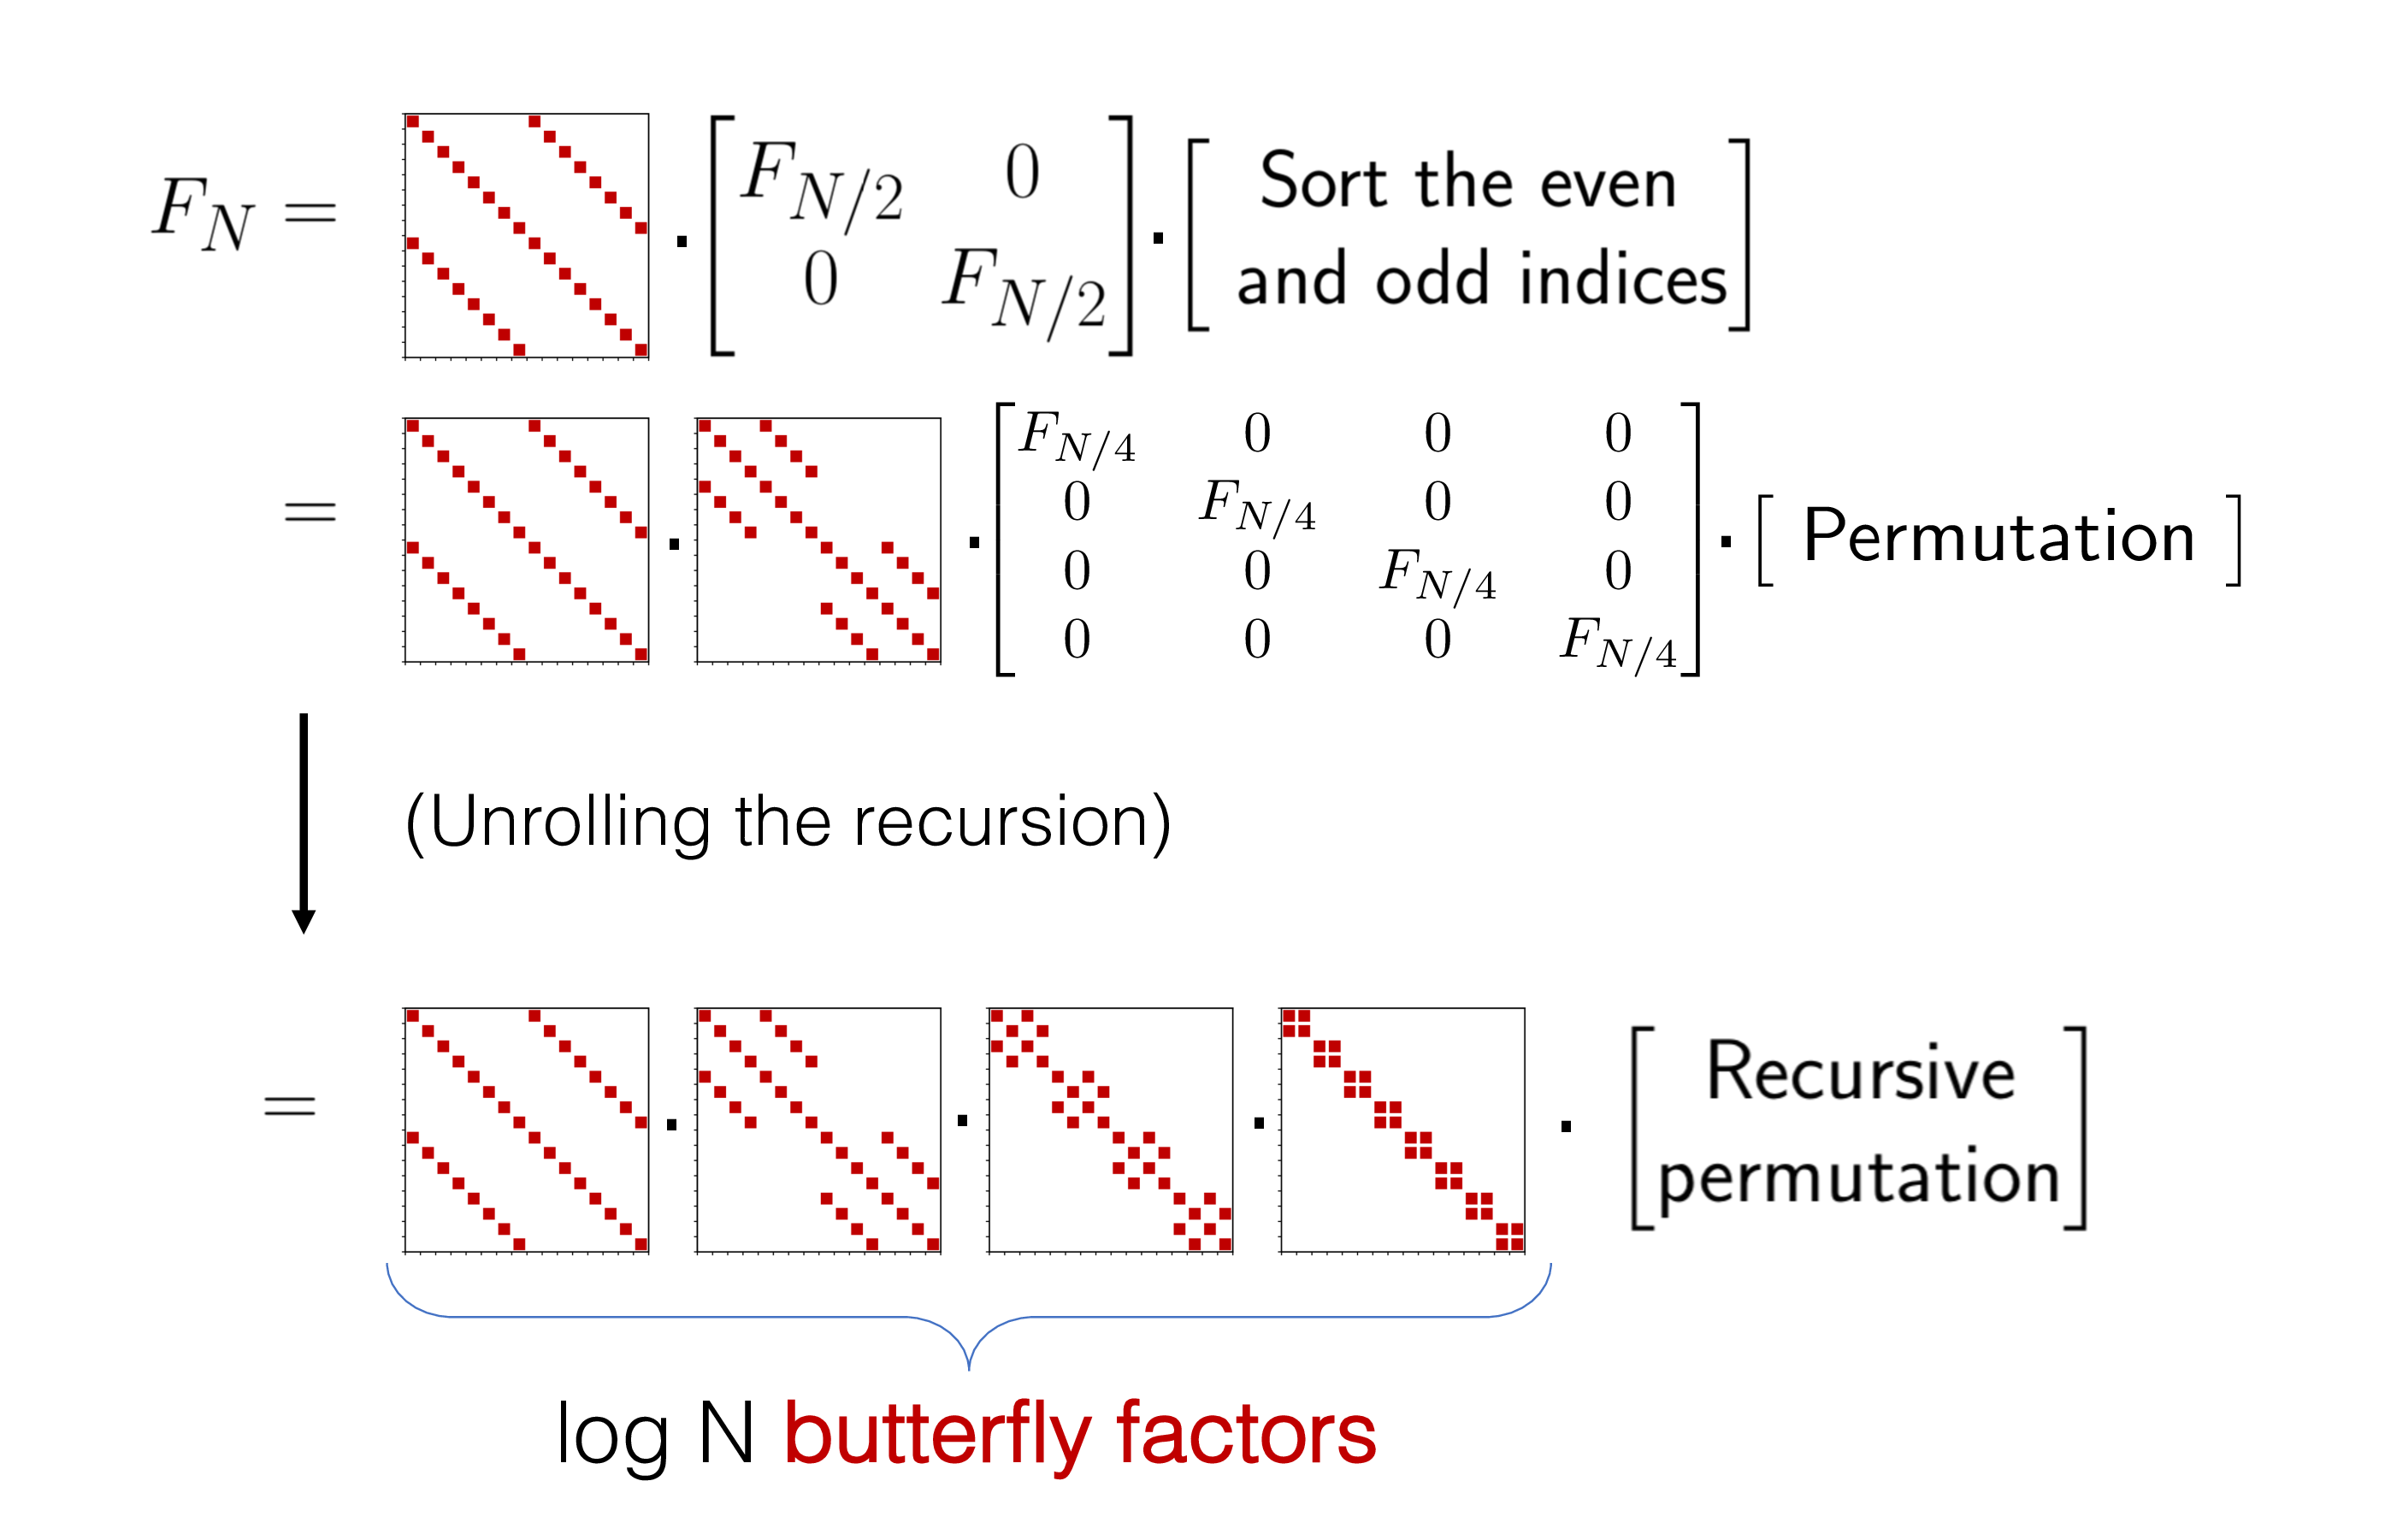
\includegraphics[width=0.32\linewidth]{f/butterflies.png} &
	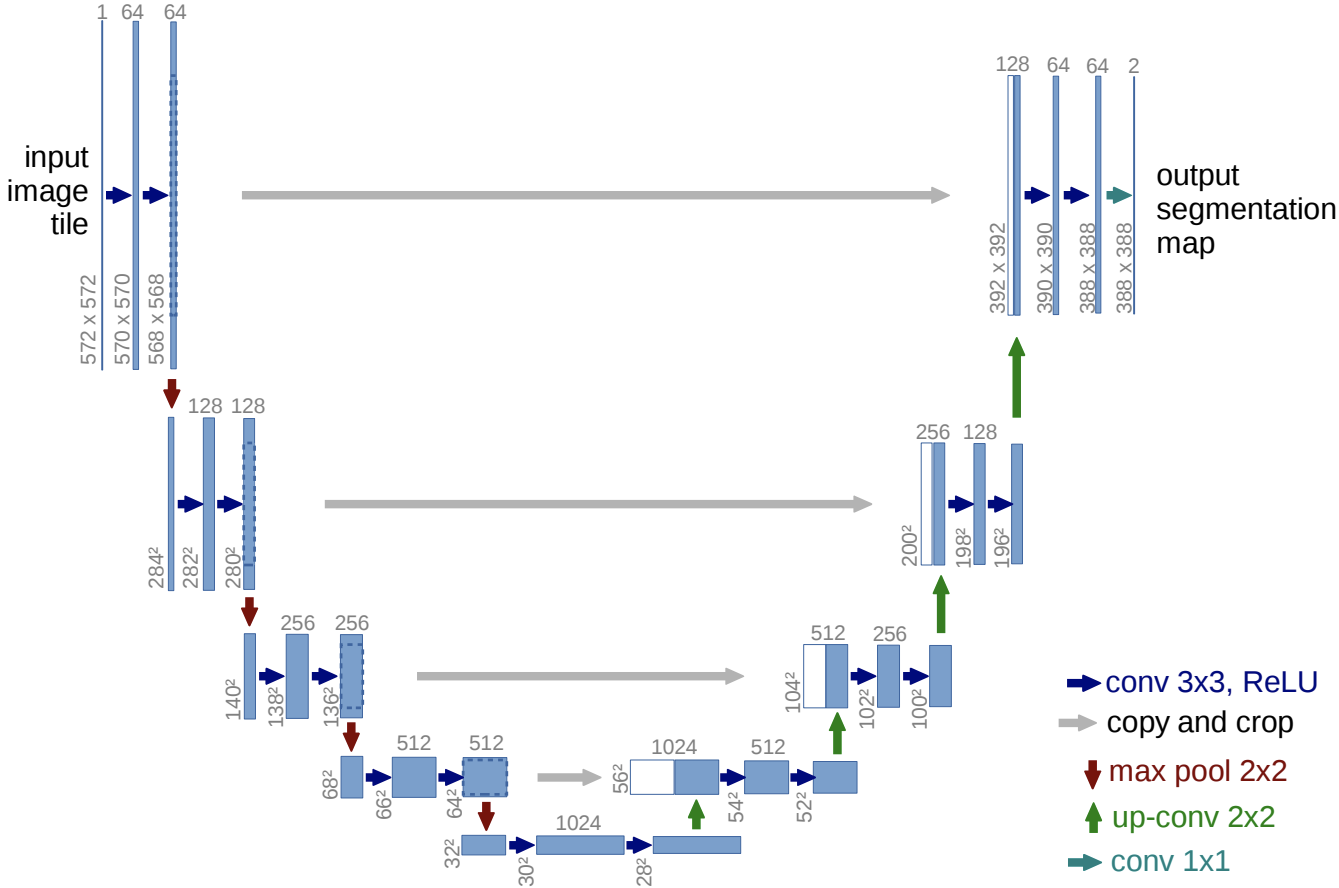
\includegraphics[width=0.32\linewidth]{f/cunet.png} \\
\end{tabular}


{\bf Objectif du stage}\\
L'objectif du stage est de creuser le plus au fond possible sur cette
correspondance.  D'abord,


%\setlength{\tabcolsep}{0pt}
%\begin{tabular}{ccccccccccc}
%	\includegraphics[width=0.093\linewidth]{f/marsmooth.png} &
%	\includegraphics[width=0.093\linewidth]{f/marbords.png} &
%	\includegraphics[width=0.093\linewidth]{f/marimba_v01.png} &
%	\includegraphics[width=0.093\linewidth]{f/marimba_v02.png} &
%	\includegraphics[width=0.093\linewidth]{f/marimba_v03.png} &
%	\includegraphics[width=0.093\linewidth]{f/marimba_v04.png} &
%	\includegraphics[width=0.093\linewidth]{f/marimba_v05.png} &
%	\includegraphics[width=0.093\linewidth]{f/marimba_v06.png} &
%	\includegraphics[width=0.093\linewidth]{f/marimba_v07.png} &
%	\includegraphics[width=0.093\linewidth]{f/marimba_v08.png} &
%	\includegraphics[width=0.093\linewidth]{f/marimba_v09.png} \\
%	$1\!\!1_\Omega$  & $W$ &
%	$\varphi_1$ &
%	$\varphi_2$ &
%	$\varphi_3$ &
%	$\varphi_4$ &
%	$\varphi_5$ &
%	$\varphi_6$ &
%	$\varphi_7$ &
%	$\varphi_8$ &
%	$\varphi_9$
%\end{tabular}


\vspace{-1.5em}
\renewcommand{\refname}{\normalsize Références}
%
\begin{thebibliography}{99}
\vspace{-1em}
{\scriptsize
\bibitem{drum}
	Kac, M..
	{\it Can one hear the shape of a drum?}
	The american mathematical monthly, (1966)

\bibitem{inverse}
	Chu, M., \& Golub, G.
	{\it Inverse eigenvalue problems: theory, algorithms, and
	applications}, OUP (2005)

\bibitem{localfun}
	Nguyen, B. \& Grebenkov, D.~S.
	{\it Localization of Laplacian eigenfunctions in circular, spherical
	and elliptical domains}, SIAM J.  Appl. Math. (2019)

\bibitem{geofun}
	Grebenkov, D.~S.  \& Nguyen, B.
	{\it Geometrical structure of Laplacian eigenfunctions},
	SIAM Rev. (2013)

\bibitem{backeigen}
	Wang,~W., Dang,~Z., Hu,~Y., Fua,~P., Salzmann,~M.
	{\it Backpropagation-Friendly Eigendecomposition},
	NeurIPS (2019)

}
\end{thebibliography}



\end{document}  


% vim:set tw=79 spell spelllang=fr:
